\section{Introduction}

The rapid advancement of aerospace technology and urban infrastructure is driving the emergence of \gls{UAM} and autonomous airliners, reshaping the future of air transportation.
\Gls{UAM} refers to the use of \gls{eVTOL} aircraft to provide efficient, low-emission air travel within and around cities, aiming to alleviate ground traffic congestion and reduce travel times \cite{easa_uam}.
Simultaneously, the development of autonomous airliners (capable of operating with minimal or no human intervention) is gaining momentum, promising increased safety, operational efficiency, and cost-effectiveness in commercial aviation \cite{Vance_2019}.
Together, these innovations mark a significant shift toward smarter, more sustainable air transportation systems, supported by breakthroughs in \gls{AI}, sensor technology, and regulatory evolution. 

As the skies grow increasingly crowded with traditional aircraft, drones, and emerging \gls{eVTOL} vehicles, modernising \gls{ATM} systems becomes essential.
Traditional \gls{ATM} frameworks, designed for conventional aviation, are not equipped to handle the complexity and volume introduced by \gls{UAM} and autonomous operations \cite{Schuchardt_2023}.
To address this, the development of \gls{UTM} has emerged as a complementary solution, enabling the safe, scalable, and efficient integration of low-altitude, autonomous air traffic into national airspace systems \cite{Singh_2024}.
\Gls{UTM} leverages digital communication, real-time data sharing, and dynamic airspace access.
Together, \gls{ATM} and \gls{UTM} form the backbone of future-proofed aerial ecosystem, ensuring safety, reliability, and coordination across all types of airborne vehicles.

% Despite the promising potential of \gls{UTM}, integrating it seamlessly into legacy \gls{ATM} systems presents significant challenges.
% One of the primary issues is the technological and procedural gap between legacy air traffic infrastructure and the digital, decentralised nature of \gls{UTM} frameworks.
% Ensuring interoperability, real-time data exchange, and cohesive traffic coordination between manned and unmanned aircraft requires robust standards, secure communication protocols, and regulatory harmonisation.
% Compounding these challenges is the ongoing global shortage of \glspl{ATCO}, which places additional strain on already overburdened \gls{ATM} operations.
% This staffing deficit not only affects the efficiency of current airspace management but also limits the capacity to oversee and adapt to the influx of new air traffic types.
% Briding the gap between \gls{UTM} and \gls{ATM} will require collaborative efforts across industry stakeholders, regulaatory bodies, and technological innovators to build a resilient, scallable system capable of supporting the future of autonomous and \gls{UAM}.

Integrating \gls{UTM} into existing \gls{ATM} infrastructure presents a range of technical, operational, and organisational challenges \cite{Singh_2024}.
Traditional \gls{ATM} systems are already under pressure, with many countries facing a critical shortage of \glspl{ATCO}: an issue that hampers the capacity to manage even current levels of air traffic safely and efficiently \cite{eurocontrol2024digitalisation}.
Adding to this challenge is the rapid growth of \gls{UAS} and \gls{UAM} operations, which introduces unpredictable flight patterns, higher traffic density in low-altitude airspace, and the nead for real-time, automated coordination \cite{Ramachandran_2025}.
These factors demand that \gls{UTM} systems be not only interoperable with legacy \gls{ATM} systems, but also highly robust, adaptive, and capable of autonomous decision-making.
Ensuring seamless integration while maintaining safety, realiabiity, and trust across both manned and unmanned aviation domains remains a core hurdle in realising the potential of next-generation air mobility.



% \subsection{Urban Air Mobility (UAM)}

According to \gls{EASA}, \gls{UAM} refers to an air transportation system for passengers and cargo in urban environments.%, with the transportation performed by an electric aircraft capable of \gls{VTOL}, either remotely piloted or with a pilot on board \cite{easa_uam}. 
It primarily consists of \gls{eVTOL} aircrafts, with air taxis used for passengers and drones for delivery of cargos, surveillance, and photography. 
These aircrafts can either be remotely piloted or with a pilot on board \cite{easa_uam}. 
If these aircrafts are capable of autonomous flying, it is considered a part of \gls{UAV}.
% \subsection{Autonomous Airliners (AA)}

Autonomous airliners represent a branch of \glspl{UAV}, consisting of fixed-wing aircraft capable of flying and navigating without direct intervention of a human pilot, for passenger service.
Although modern commercial airliners already automate approximately 93\% of flight functions, there remains a growing demand to implement higher levels of autonomy  \cite{Vance_2019}.
Increased automation is seen as a path toward enhanced safety, greater scalability, and improved affordability.

% \subsection{Differences between UAM, AA and UAV}

\Gls{UAM} differs from traditional aircrafts with its use of rotors, and the ability to take off and land vertically from almost anywhere with a suitable platform, such as vertiports, and helipads, whereas traditional aircrafts are mostly equipped with fixed wings and require runways to operate \cite{Schuchardt_2023}.
Its range of opperation also differs, with \gls{UAM} operate in urban areas (intra- and inter-city) while traditional aircrafts are able to operate for long distance travel, but only to locations with runway availability.
Fig.~\ref{fig:venn-diagram} shows the comparison between \gls{UAM}, \gls{UAV} and conventional aircrafts.
Fig.~\ref{fig:airspace-mobility} shows the distance which the aircrafts travel to and from, as well as the airspace it occupies.

\begin{figure}[h]
    \centering
    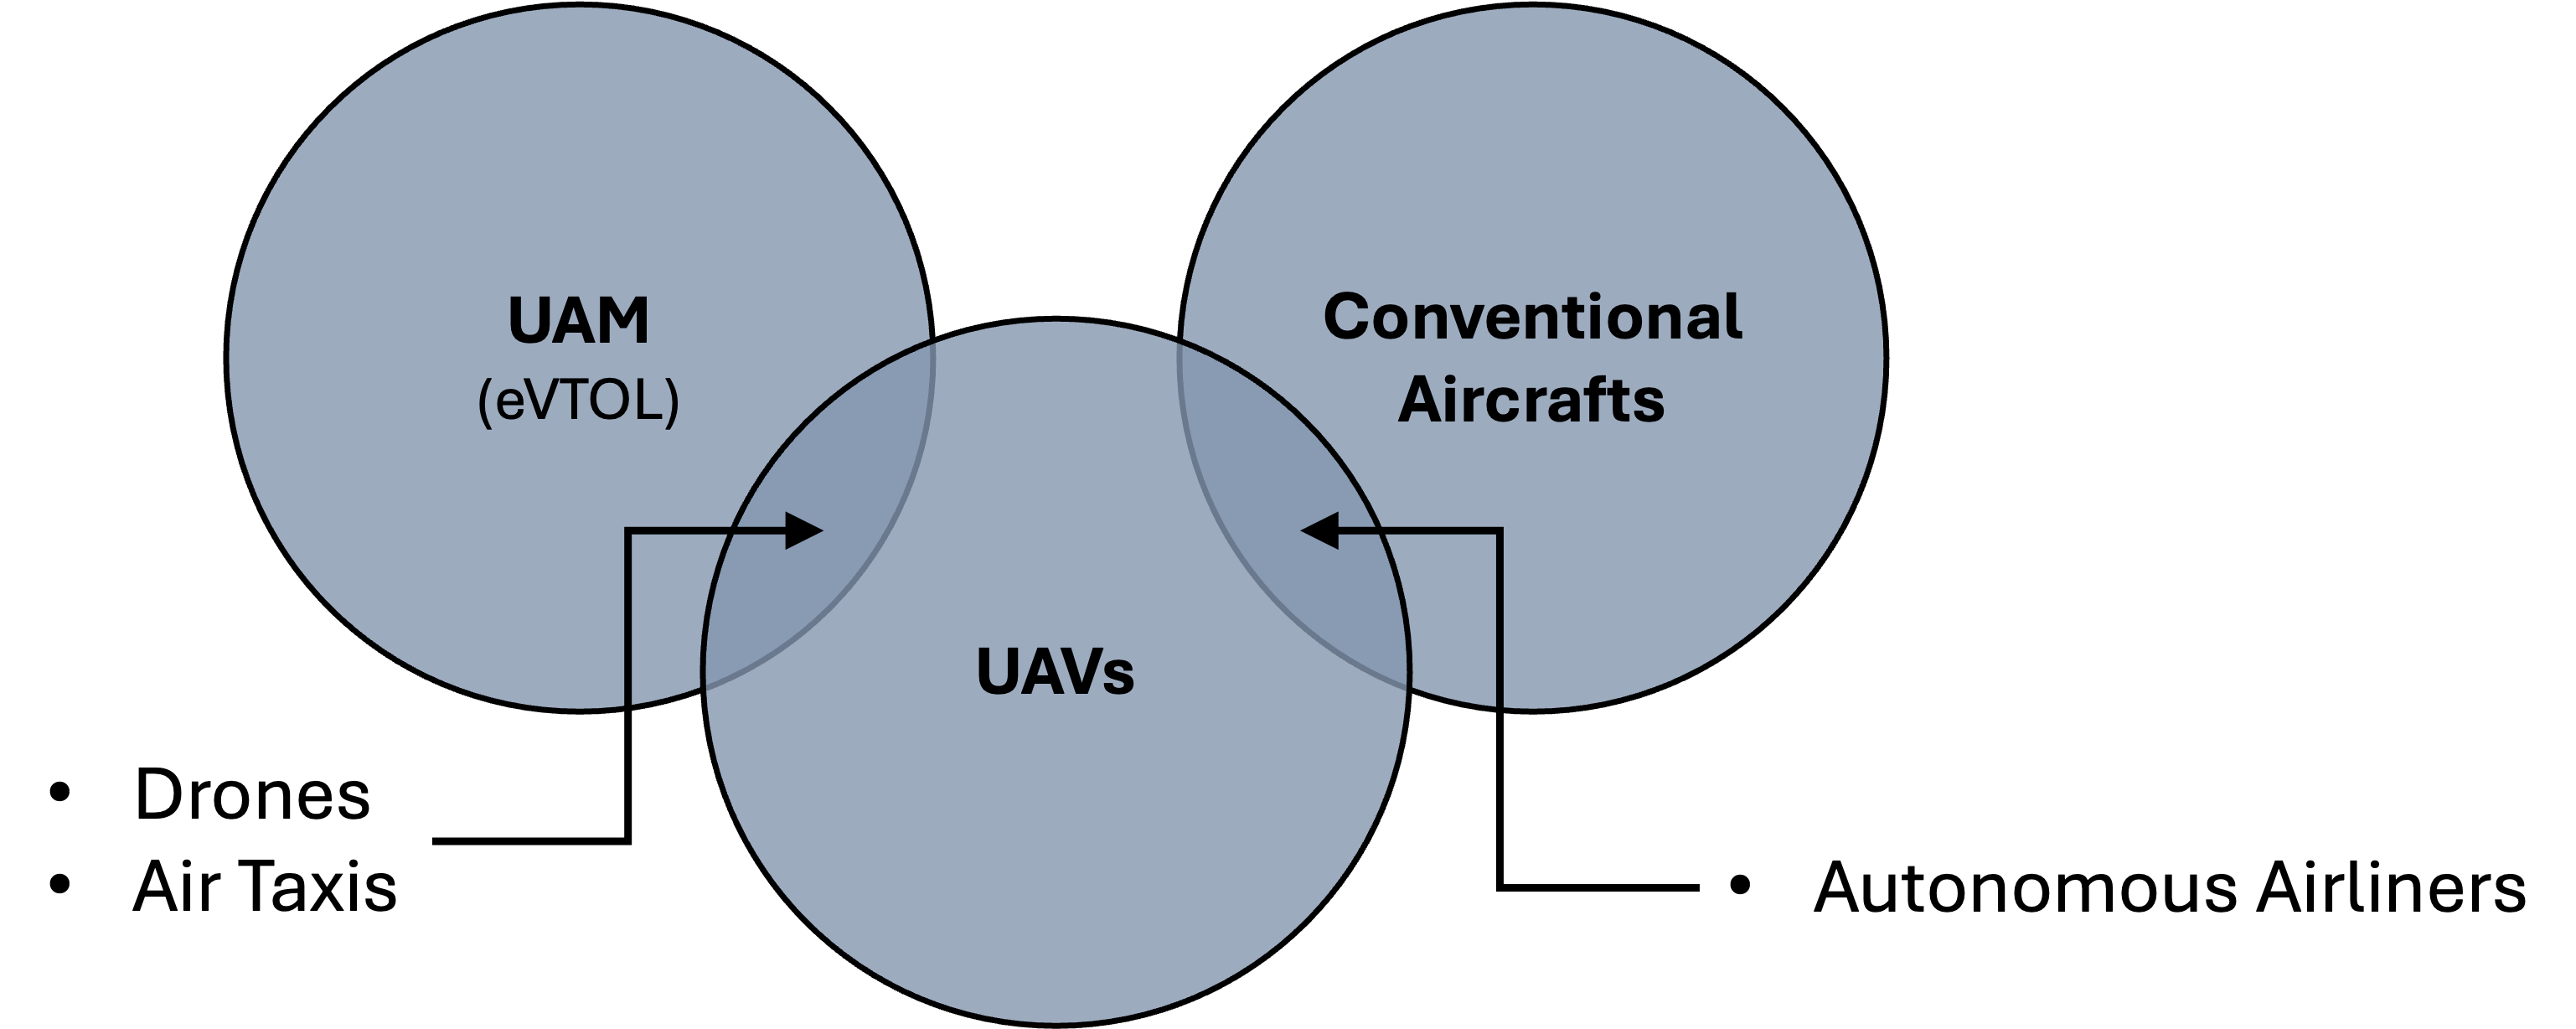
\includegraphics[width=.6\textwidth]{venn-diagram.png}
    \caption{Venn diagram of \gls{UAM}, \gls{UAV} and conventional aircrafts.}
    \label{fig:venn-diagram}
\end{figure}

\begin{figure}[h]
    \centering
    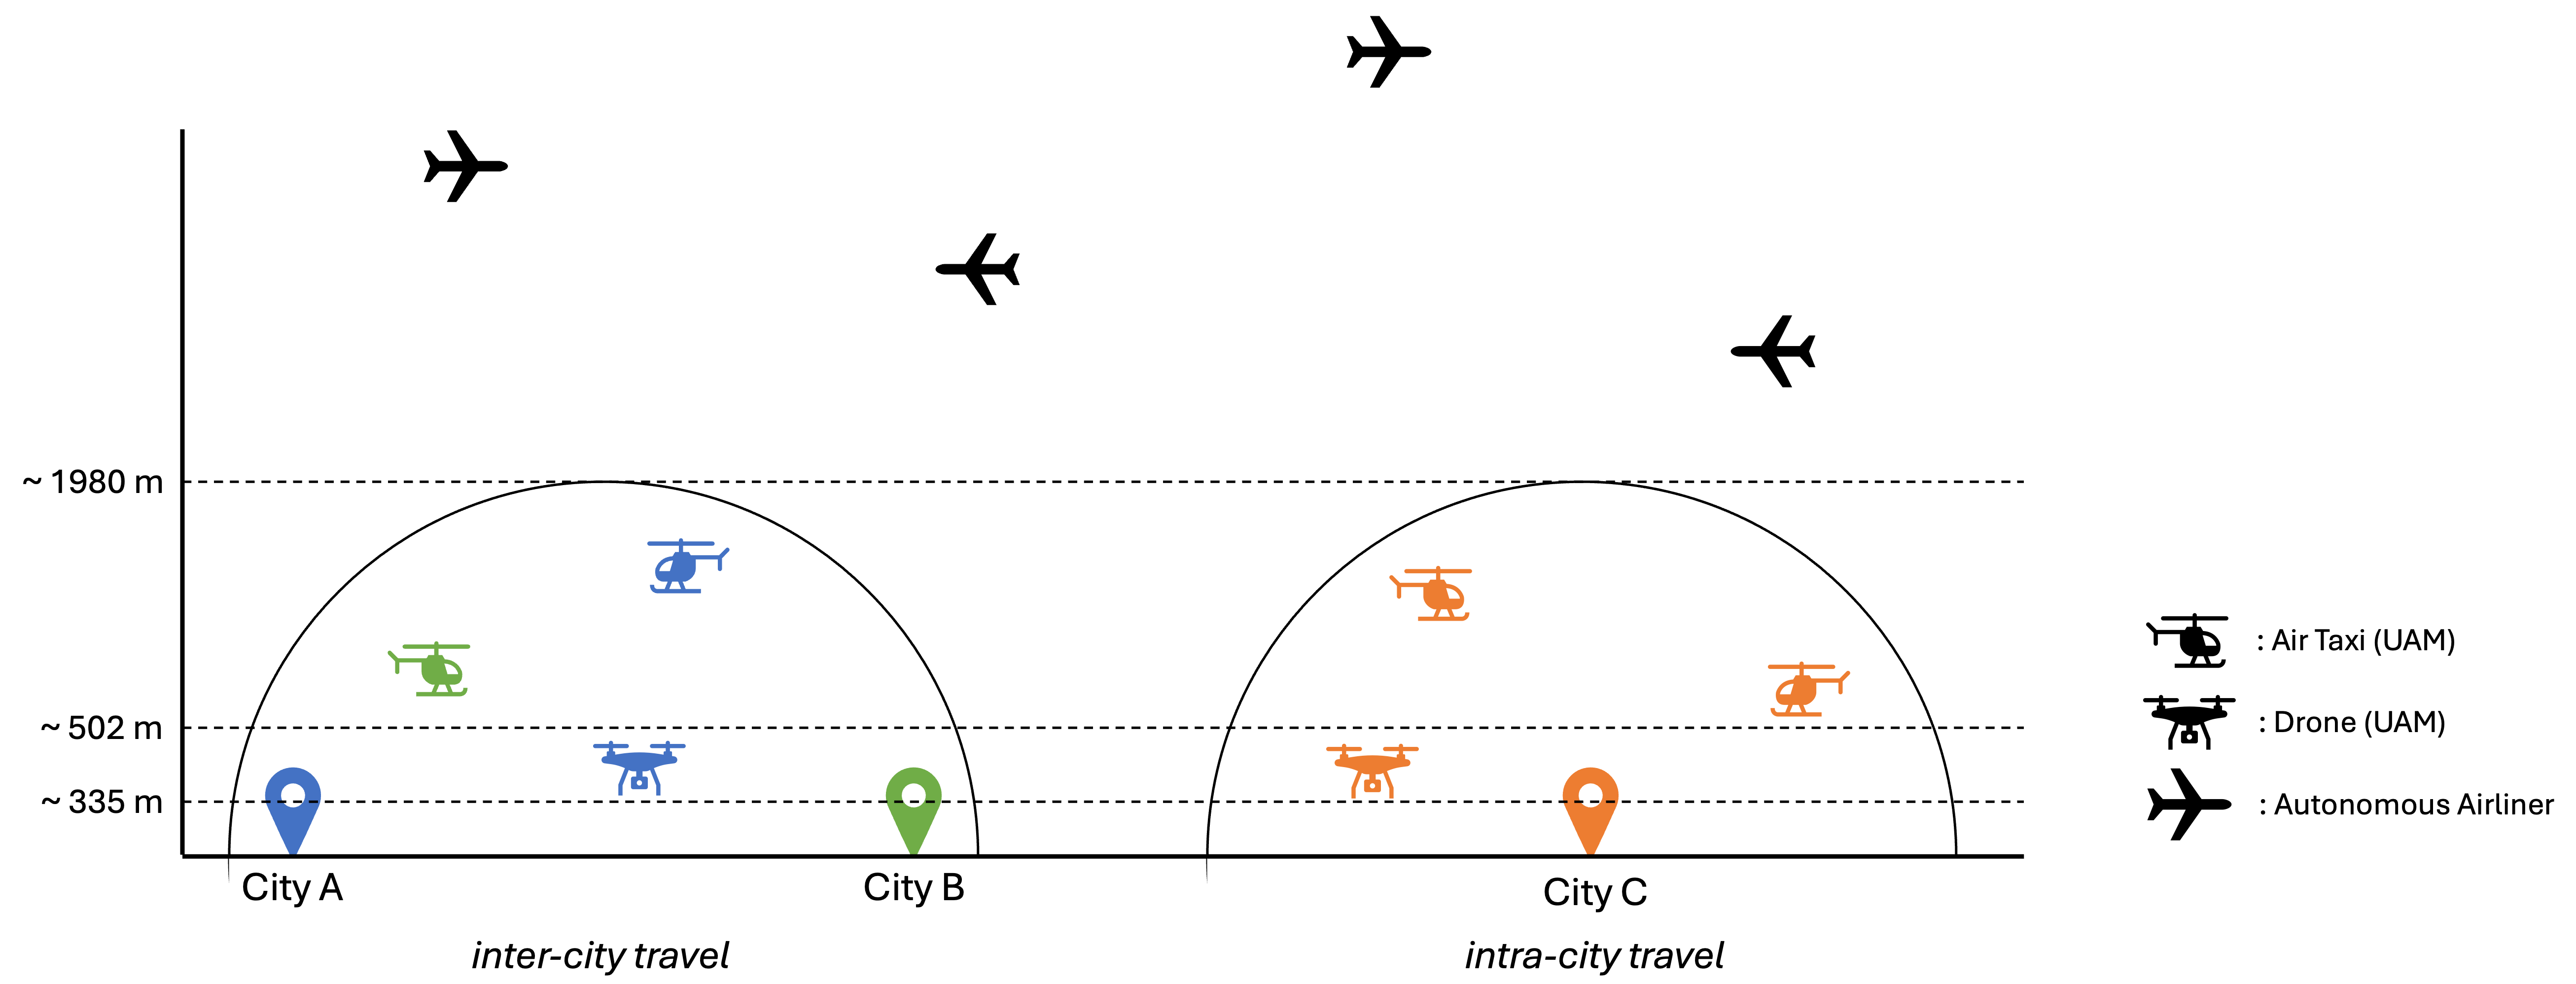
\includegraphics[width=\textwidth]{airspace-mobility.png}
    \caption{Mobility of \gls{UAM} and autonomous airliners.}
    \label{fig:airspace-mobility}
\end{figure}

% \subsection{Air Traffic Management (ATM)}

\Gls{ATM} is the aggregation of the airborne and ground-based functions required to ensure the safe and efficient movement of aircraft during all phases of operations, through controlled airspaces and on the ground at airports \cite{skybraryATM}.
It comprises serveral components, including \gls{ATS}, \gls{ASM}, and \gls{ATFM} \cite{skybraryATM}.
Figure \ref{fig:atm-structure} shows the structure of \gls{ATM} and the relationship between \gls{ATS}, \gls{ASM}, and \gls{ATFM}.

\begin{figure}[h]
    \centering
    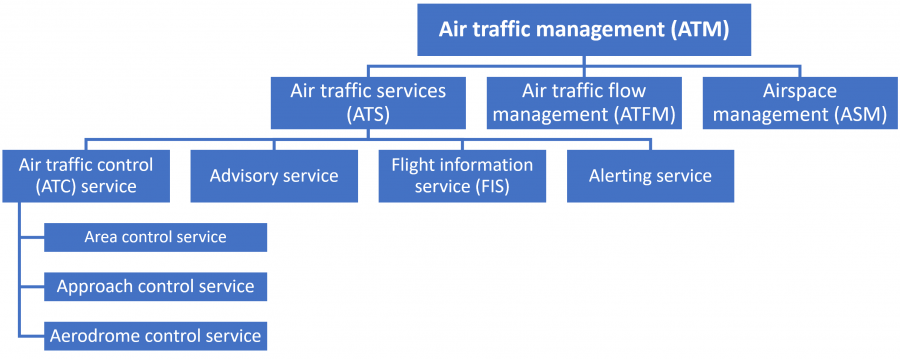
\includegraphics[width=0.8\linewidth]{900px-ATM_Chart.png}
    \caption{Structure of \gls{ATM} \cite{skybraryATM}}
    \label{fig:atm-structure}
\end{figure}

\Glspl{ATCO}, part of \gls{ATC} service, are responsible for directing aircraft safely and efficiently, managing takeoffs and landings, maintaining safe distances between aircraft en route and handling emergencies. 
Their role demands high levels of situational awareness, rapid decision-making, and the ability to manage multiple tasks under high stress conditions.
These indispensable skills, such as judgement, flexibility and the ability to handle unexpected situations, remains critical and are not easily replicated by automated systems \cite{eurocontrol2024digitalisation}.
% \subsection{UAS Traffic Management (UTM)}

\Gls{UTM} is a system for safely managing \gls{UAV} operations at low altitude. 
Separate from but complementary to \gls{ATS}, it enables fucntions such as flight planning, authorisation, surveillance, and conflicht management to mitigate risks and ensure safe, efficient operations of \glspl{UAV}.
There is ongoing work to fully realize the benefits of \gls{UTM} \cite{faa_utm}.
% \subsection{Challenges of integrtaing UTM with ATM}

Integrating \gls{UTM} into traditional \gls{ATM}is complex but crucial for ensuring safe and efficient airspace operations, primary due to the differing nature of \gls{UAS} and manned aircrafts. 
While \gls{UTM}, designed to manage drone missions, , it must be integrated seamlessly into the existing \gls{ATM} infrastructure to prevent accidents and enhance scalability. 
Both systems must work together, as unmanned flight systems need to detect and respond to other aircraft in emergencies, and vice versa \cite{flynex2020utm_atm}.

The growing complexity of \gls{ASM}, driven by the driven by the rapid expansion of commercial aviation, \gls{UAM}, and \glspl{UAV}, has led to increased air traffic volume.
As air traffic rises, and with the limited capacity of \glspl{ATCO} highlight the need for AI-based solutions, such as real-time data processing and predictive analytics, to improve system performance \cite{Ramachandran_2025}.
Despite existing automation, current systems often rely on rigid frameworks that lack the flexibility needed for dynamic environments  \cite{Meier_2024}.

Additionally, \gls{UAS} have unique performance characteristics that complicate their integration into the air traffic flow, often resulting in suboptimal use of airspace capacity.
\Glspl{UAV} typically operate across both controlled and uncontrolled airspaces, and since \glspl{ATCO} only manage controlled spaces, the lack of oversight in uncontrolled airspace raises the risk of collisions or accidents. 
As a result, \gls{UTM} systems are essential for ensuring safe and efficient \gls{UAV} operations across all airspaces \cite{Zsolt_2017}, highlighting the urgent need for scalable, flexible, and automated solutions in air traffic management.
% \subsection{Objective}